% Template for Cogsci submission with R Markdown

% Stuff changed from original Markdown PLOS Template
\documentclass[10pt, letterpaper]{article}

\usepackage{cogsci}
\usepackage{pslatex}
\usepackage{float}
\usepackage{caption}

% amsmath package, useful for mathematical formulas
\usepackage{amsmath}

% amssymb package, useful for mathematical symbols
\usepackage{amssymb}

% hyperref package, useful for hyperlinks
\usepackage{hyperref}

% graphicx package, useful for including eps and pdf graphics
% include graphics with the command \includegraphics
\usepackage{graphicx}

% Sweave(-like)
\usepackage{fancyvrb}
\DefineVerbatimEnvironment{Sinput}{Verbatim}{fontshape=sl}
\DefineVerbatimEnvironment{Soutput}{Verbatim}{}
\DefineVerbatimEnvironment{Scode}{Verbatim}{fontshape=sl}
\newenvironment{Schunk}{}{}
\DefineVerbatimEnvironment{Code}{Verbatim}{}
\DefineVerbatimEnvironment{CodeInput}{Verbatim}{fontshape=sl}
\DefineVerbatimEnvironment{CodeOutput}{Verbatim}{}
\newenvironment{CodeChunk}{}{}

% cite package, to clean up citations in the main text. Do not remove.
\usepackage{apacite}

% KM added 1/4/18 to allow control of blind submission


\usepackage{color}

% Use doublespacing - comment out for single spacing
%\usepackage{setspace}
%\doublespacing


% % Text layout
% \topmargin 0.0cm
% \oddsidemargin 0.5cm
% \evensidemargin 0.5cm
% \textwidth 16cm
% \textheight 21cm

\title{Pressure to communicate across knowledge asymmetries leads to
pedagogical-like language input}


\author{{\large \bf Benjamin C. Morris} \\ \texttt{benmorris@uchicago.edu} \\ Department of Psychology \\ University of Chicago \And {\large \bf Daniel Yurovsky} \\ \texttt{yurovsky@uchicago.edu} \\ Department of Psychology \\ University of Chicago}

\begin{document}

\maketitle

\begin{abstract}
Infants prefer to listen to and learn better from child-directed speech.
This speech might support learning in part due to communicative
pressure: parents must use language that their children understand. We
present longitudinal corpus data of parent-child interaction to
demonstrate that parents provide information-rich referential
communication (using both gesture and speech during the same reference)
more for infrequent referents and when their children are younger. We
then present a Mechanical Turk study to experimentally validate this
idea, asking Turkers to communicate with a listener who a novel language
less well. Participants could communicate in 3 ways: pointing (expensive
but unambiguous), labelling (cheap but knowledge-dependent), or both.
They won points only for communicating successfully; using pointing and
labelling together was costly, but could teach, allowing cheaper
communication on later trials. Participants modulated their
communicative behavior in response to their own and their partner's
knowledge and teaching emerged when the speaker had substantially more
knowledge of the lexicon. While language is more than reference games,
this work validates the hypothesis that communicative pressure alone can
lead to supportive language input.

\textbf{Keywords:}
Language; Learning; Child-Directed Speech; POMDP.
\end{abstract}

\section{Introduction}\label{introduction}

One of the most striking aspects of children's language learning is just
how quickly they master the complex system of their natural language
(Bloom, 2000). In just a few short years, children go from complete
ignorance to conversational fluency in a way that is the envy of
second-language learners attempting the same feat later in life
(Newport, 1990). What accounts for this remarkable transition?

One possibility is that children's caregivers deserve most of the
credit; that the language parents produce to their children is optimized
for teaching. Although there is some evidence that aspects of
child-directed speech support learning, other aspects--even in the same
subproblem, e.g.~phoneme discrimination--appear to make learning more
difficult (Eaves Jr, Feldman, Griffiths, \& Shafto, 2016; McMurray,
Kovack-Lesh, Goodwin, \& McEchron, 2013). In general, parents rarely
explicitly correct their children, and children are resistant to the
rare explicit language correction they do get (Newport, Gleitman, \&
Gleitman, 1977). Thus while parents may occasionally offer a supervisory
signal, the bulk of the evidence suggests that parental supervision is
unlikely to explain rapid early language acquisition

Alternatively, even the youngest infants may already come to language
acquisition with a precocious ability to learn the latent structure of
language from the statistical properties of speech in their ambient
environment (Saffran \& 2003, 2003; L. B. Smith \& Yu, 2008). While a
number of experiments clearly demonstrate the early availability of such
mechanisms, there is reason to be suspicious about just how precocious
they are early in development. For example, infants' ability to track
the co-occurrence information connecting words to their referents
appears to be highly constrained by both their developing memory and
attention systems (L. B. Smith \& Yu, 2013; Vlach \& Johnson, 2013).
Further, computational models of these processes show that the rate of
acquisition is highly sensitive to variation in environmental statistics
(Blythe, Smith, \& Smith, 2010; Vogt, 2012). Thus precocious
unsupervised statistical learning also appears to fall short of an
explanation for rapid early language learning.

We explore the consequences of a third possibility: The language that
children hear is neither designed for pedagogy, nor is it random; it is
designed for communication (Brown, 1977). We take as the caregiver's
goal the desire to communicate with the child, not about language
itself, but instead about the world in front of them. To succeed, the
caregiver must produce the kinds of communicative signals that the child
can understand, and thus might tune the complexity of their speech not
for the sake of learning itself, but as a byproduct of in-the-moment
pressure to communicate successfully (Yurovsky, 2017).

To examine this hypothesis, we first analyze parent communicative
behavior in a longitudinal corpus of parent-child interaction in the
home (Goldin-Meadow et al., 2014). We investigate the extent to which
parents modify their communicative behavior across their child's
development to align to their child's developing linguistic knowledge.
\textbf{?maybe something about alignment at other levels, syntatic,
lexical, etc.,--\textgreater{} but we're looking here for modality?}
Specifically, we analyze communicative modality to look for instances
multi-modal reference-- when speakers indicate the same referent, in the
same instance, using both gesture and a verbal label. These instances
might be particularly powerful learning opportunities for young children
because they provide a verbal label in the presence of a highly
disambuiguting gestural cue (e.g., pointing, holding), greatly reducing
referential uncertainty (\textbf{gesture-speech citation, word-learning
as uncertainty reduction}).

We then turn to the emergence of structured input in a simple model
system: an iterated reference game in which two players earn points for
communicating successfully with each other. Modeled after our corpus
data, particpants are asked to make choices about which communicative
strategy to use (akin to modality choice). In an experiment on
Mechanical Turk using this model system, we experimentally induce
structured language input from a pressure to communicate. We then show
that human behavior can be explained by a rational planning model that
seeks to optimize its total expected utility over the course of the
game.

\section{Corpus Analysis}\label{corpus-analysis}

To begin with, we investigate linguisitc input in naturalistic,
parent-child corpus data. We focus on parent referential communication
to examine how parents might be aligning to their children. The degree
of parental alignment should be sensitive to the child's age, such that
parents will be more likely to provide richer communicative information
when their child is younger, when she has less linguistic knowedge, than
as she gets older (Yurovsky, Doyle, \& Frank, 2016). Parental alignment
should also be stronger for infrequent objects, where again children are
likely to have less knowledge of the relevant label. We analyze the
production of multi-modal reference for the same referent, in the same
instance, which could reflect alignment if parents are senstively using
this information-rich cue for young children and infrequent objects.

\subsection{Data}\label{data}

These data come from the Language Development Project, a large-scale,
longitudinal corpus of parent child-interaction in the home with
families who are representative of the Chicago community in
socio-economic, racial, and gender diversity (\textbf{Goldin-Meadow et
al., 2014})\ldots{} \textbf{add specific demographics info}

These data are drawn from a sample of 10 families from the greater
corpus. Recordings were taken in the home every 4-months from when the
child was 14-months-old until they were 34-months-old, resulting in 6
timepoints (missing one family at the 30-month timepoint). Recordings
were 90 minute sessions, and participants were given no instructions.

\paragraph{Corpus Coding}\label{corpus-coding}

The Language Development Project corpus contains transcription of all
speech and communicative gestures produced by children and their
caregivers over the course of the 90-minute home recordings. An
independent coder analyzed each of these communicative instances and
identified each time a concrete noun was referenced using speech (i.e.,
a specific noun form), gesture (only deictic gestures were coded for
ease of coding and interpretation-- e.g., pointing) or both
simultaneously.

\subsection{Results}\label{results}

These corpus data were analyzed using a mixed effects regression to
predict parent use of multi-modal reference for a given referent. Random
effects of subject and referent were included in the model. Our key
predictors were child age and referent frequency as a spoken token in
the corpus overall.

We find a signficant negative effect of age on multi-modal reference,
such that parents are signficantly less likely to provide the
gesture-speech cue as their child gets older (\emph{B \textless{}}
-0.038, \emph{p \textless{} 0.0001}). Examing referents, we find a
signficant negative effect of referent frequency on multi-modal
reference as well, such that parents are signficantly less likely to
provide the gesture-speech cue for frequent referents than infrequent
ones (\emph{B \textless{}} -0.13, \emph{p \textless{} 0.0001}). Thus, in
these data, we see early evidence that parents are providing richer,
structured input about rarer things in the world for their younger
children.

\begin{CodeChunk}
\begin{figure}[tb]

{\centering 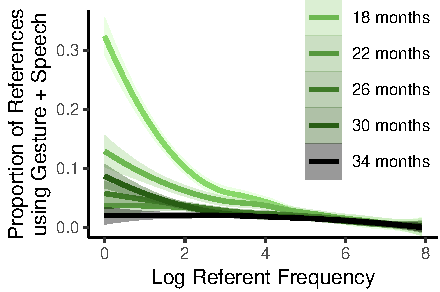
\includegraphics{figs/corpus_plot-1} 

}

\caption[Proportion of parent referential talk with speech-gesture cooccurence across development]{Proportion of parent referential talk with speech-gesture cooccurence across development. Lines represent child's age (14-34 months). The log of the referent's frequency is given on the x-axis, with more infrequent items closer to zero.}\label{fig:corpus_plot}
\end{figure}
\end{CodeChunk}

\subsection{Discussion}\label{discussion}

We have shown that parents provided more multi-modal reference for less
familiar objects and when their child is younger. These corpus findings
are consistent with an account of parental alignment: parents are
sensitive to their child's developing linguisitc knowledge and adjust
their communicative behavior accordingly. Alignment may be one example
of the pressure to communicate sucessfully in the moment leading to
richly-structured language input; however, with naturalistic data it is
difficult to determine the role of the underlying pressures at work.
While these data are consistent with our account of the role of
communicative pressure and alignment, these data could also result from
(\textbf{any number of pressures, from pedagogical to\ldots{} }). To
take our ideas further, we next developed a paradigm to try to
experimentally induce richly-structured, aligned input from a pressure
to communicate in the moment, as a proof of concept.

\section{Experimental Framework}\label{experimental-framework}

To study the emergence of pedagogical-like input from communicative
pressure, we developed a simple reference game in which participants
would be motivated to communicate successfully on a trial-by-trial
basis. By manipulating the relative costs of the communicative methods
and examining the role of differential knowledge states, we aim to
determine the circumstances under which richly-structured input emerges,
without an explicit pedagogical goal. If people are motivated to
communicate successfully, their choice of referential modality should
reflect the tradeoff between the cost of producing the communicative
signal with the likelihood that the communication would succeed. In all
conditions, pariticpants are placed in the role of speaker and asked to
communicate with a computerized listner whose responses were programmed
to be contingent on speaker behavior.

\subsection{Method}\label{method}

\subsubsection{Participants}\label{participants}

480 participants were recruited though Amazon Mechanical Turk and
received a \$1 payment for their participation. Data from 51
participants were excluded from subsequent analysis for failing the
critical manipulation check and a further 28 for producing
pseudo-English labels (e.g., `pricklyyone'). \textbf{add footnote that
analyses were done with and without these participants and patterns
hold?}

\subsubsection{Design and Procedure}\label{design-and-procedure}

Participants were told they would be introduced to novel object-label
pairs and then asked to play a communication game with a partner.
Participants were exposed to nine novel objects, each with a randomly
assigned pseudo-word label. We manipulated the degree of exposure within
subjects, such that, during training participants saw three of the nine
object-label mappings four times, two times, or one time. Thus,
particpants had a total of 20 training trials. Participants were then
given a simple recall task to establish their baseline knowledge of the
novel lexicon (pretest).

\begin{CodeChunk}
\begin{figure}[H]

{\centering 
\includegraphics{figs/exp_screenshot-1} 

}

\caption[Screenshot of speaker view during gameplay]{Screenshot of speaker view during gameplay.}\label{fig:exp_screenshot}
\end{figure}
\end{CodeChunk}

Prior to beginning the game, participants are told how much exposure
their partner has had to the lexicon and also that they will be asked to
discuss each object three times. Participants are then asked to report
their partner's level of exposure, and are corrected if they answer
wrongly (manipulation check). Then during gameplay, speakers saw a
target object in addition to an array of all nine objects (see Figure
\ref{fig:exp_screenshot} for the speaker's perspective). Speakers had
the option of either directly selecting the target object from the array
(gesture)- a higher cost cue but without ambiguity- or typing a label
for the object (speech)- a lower cost cue but contingent on the
listener's shared linguistic knowledge. After sending the message,
speakers are shown which object the listener selected.

Speakers could win up to 100 points per trial if the listener correctly
selected the target referent based on their message. We manipulated the
relative utilities of each of the strategies between-subjects across two
conditions: `Talk is Cheap' and `Talk is Less Cheap.' In the `Talk is
Cheap' condition, sending a message by gesturing cost 70 points while
sending a label cost 0 points, yielding 30 points and 100 points
respectively if the listner selected the target object. In the `Talk is
Less Cheap' condition speakers were charged 50 points for gesturing and
20 points for labeling, yielding up to 50 points and 80 points
respectively. If the listener failed to identify the target object, the
speaker nevertheless paid the relevant cost for that message in that
condition. As a result of this manipulation, there was a higher relative
expected utilty for labeling in the `Talk is Cheap' conditon than the
`Talk is Less Cheap' condition.

Critically, particpants were told about a third type of possible message
using both gesture and speech within a single trial to effectively teach
the listener an object-label mapping. This action directly mirrors the
multi-modal reference behavior from our corpus data-- it presents the
listener with an information-rich, potentially pedagogical learning
moment. In order to produce this teaching behavior, speakers had to pay
the cost of producing both cues (i.e.~both gesture and speech). Note
that, in both utility conditions, teaching nets participants 30 points.
Our communicative game was designed to reward in-the-moment
communication, and thus teaching required the speaker pay a high cost
upfront. However, rational communicators may understand that if one is
accounting for future trials, paying the cost upfront to teach the
listener allows a speaker to use a less costly message strategy on
subsequent trials (namely, speech).

Incorporating teaching means that our speaker must also reason about
their interlocutor's knowledge state more explicitly, in order to make
rational decisions about what to teach and when. To address this added
dimension, we also manipulated participants' expectations about their
partner's knowledge across 3 conditions. Participants were told that
their partner had either no experience with the lexicon, had the same
experience as the speaker, or had twice the experience of the speaker.

Listeners were programmed with starting knowledge states initialized
accordingly. Listeners with no exposure began the game with knowledge of
0 object-label pairs. Listeners with the same exposure of the speaker
began with knowledge of five object-label pairs (3 high frequency, 1 mid
frequency, 1 low frequency), based the average retention rates found
previously. Lastly, the listener with twice as much exposure as the
speaker began with knowledge of all nine object-label pairs. If the
speaker produced a label, the listener was programmed to consult their
own knowledge of the lexicon and select the closest known reference
(selecting a label with a levenshtein edit distance of two or fewer from
the speaker's production). If there was not a similar known label
(i.e.~edit distance \textgreater{} 2), the lsitener was programmed to
select randomly among unknown objects. If the speaker gestured (or
taught by producing gesture and a label), the listener was programmed to
always select the gestured object. After a teaching trial, listeners
integrated the taught object-label mapping into their set of candidate
word-meanings when evaluating subesquent messages.

Crossing our two between-subjects manipulations, we had 6 conditions (2
utility condition: `Talk is Cheap' and `Talk is Less Cheap'; and 3
levels of partner's exposure: none, same, double), with 80 participants
in each condition. We expected to find results that mirrored our corpus
findings such that there would be higher rates of teaching behavior when
there was an asymmetry in knowledge where the speaker knew more (none
conditions) comapred with when there was equal knowledge (same
conditions) or when the listener was more familiar with the languauge
(double conditions). If particpants are motivated to communciate
efficiently, we expected that particpants would also be sensitive to our
utility manipulation, such that rates of labeling and teaching would be
higher in the `Talk is Cheap' conditions than the other conditions.

\subsection{Results}\label{results-1}

As expected, participants were sensitive to both the exposure rate and
the relative utilities of the communication strategies. As an initial
check of our knowledge manipulation, a logistic regression indicated
that the more exposures to a given object-label pair during training,
the more likely participants were to recall that label at pretest
(\textbf{B = XYZ, p \textless{} XYZ}). On average, participants knew at
least 6 of the 9 words in the lexicon (mean = 6.28, sd = 2.26).

\subsubsection{Gesture-Speech Tradeoff}\label{gesture-speech-tradeoff}

To determine how gesture and speech are trading off across conditions,
we looked at a mixed effects logistic regression to predict whether
speakers chose to produce a label during a given trial as a function of
the exposure rate, utility manipulation, and partner manipulation. A
random subjects effects term was included in the model. There was a
significant effect of exposure rate such that the more exposures to a
particular object-label pair during training, the more likely a speaker
was to produce a label (\emph{B =} 0.63, \emph{p \textless{} 0.0001}).
Participants also modulated their communicative behavior on the basis of
the utility manipulation and our partner exposure manipulation. Speakers
in the Talk is Cheap condition produced significantly more labels than
participants in the Talk is Less Cheap condition (\emph{B =} -0.84,
\emph{p \textless{} 0.001}). Speakers did more labeling with more
knowledable partners; compared with the listener with no exposure, there
were significantly higher rates of labeling in the same exposure
(\emph{B =} 2, \emph{p \textless{} 0.001}) and double exposure
conditions (\emph{B =} 3.47, \emph{p = 0.001}).

\textbf{should appearance \# be in this model too? it is in the teaching
model}

Thus, participants are sensitive to our manipulations, altering their
choices about how to communicate with their partner on the basis of the
degree of training, and the imposed utilities. Figure
\ref{fig:exp_speech_gesture} illustrates the gesture-speech tradeoff
pattern in the double exposure condition (where the listener has more
exposure than the speaker, as there was minimal teaching in that
condition and thus the speech-gesture trade-off is most interpretable).
Note that these effects do not merely reflect the degree of participant
knowledge; all patterns above hold when looking only at words
successfully learned by the speaker at pretest.

\textbf{also go through gesture results?}

\begin{CodeChunk}
\begin{figure}[H]

{\centering 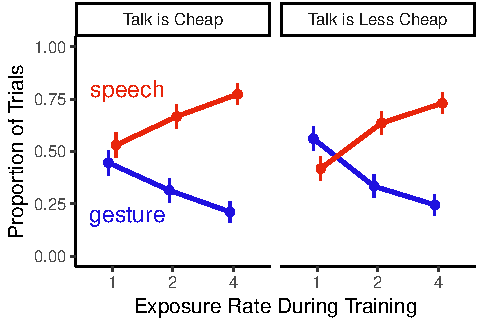
\includegraphics{figs/exp_speech_gesture-1} 

}

\caption[Speakers' communicative method choice as a function of exposure and the utility manipulation]{Speakers' communicative method choice as a function of exposure and the utility manipulation. The left panel shows the 'Talk is Cheap' condition, where typing yielded 100 points and gesturing yielded 30 points. The right panel shows the 'Talk is Less Cheap' panel where typing yielded 80 points and gesturing yielded 30 points. These data are taken only from the condition Double Exposure condition (where listeners had more exposure to the lexicon than speakers). This condition had minimal amounts of teaching, thus the speech-gesture trade-off is most easily interpreted here. Rates of teaching not show.}\label{fig:exp_speech_gesture}
\end{figure}
\end{CodeChunk}

\subsubsection{Emergence of Teaching.}\label{emergence-of-teaching.}

Thus far, we have focused on relatively straightforward scenarios to
demonstrate that a pressure to communicate successfully in the moment
can lead speakers to trade-off between gesture and speech sensibly.
Next, we turn to the emergence of teaching behavior.

In line with our hypotheses, we found that teaching is also sensitive to
same factors as the gesture-speech trade-off. A mixed effects logistic
regression predicting whether or not teaching occurred on a given trial
revealed that teaching rates across conditions depend on all of the same
factors that predict speech and gesture. There was a significant effect
of initial exposure to the mapping on the rates of teaching, such that
more exposures to a word predicted higher rates of teaching behavior
(\emph{B =} 0.16, \emph{p \textless{} 0.01}). There was also a
significant effect of the utility manipulation such that being in the
Talk is Cheap condition predicted higher rates of teaching than being in
the Talk is Less Cheap condition (\emph{B =} -0.92, \emph{p \textless{}
0.01}), a rational response considering teaching allows one to use a
less costly strategy in the future and that strategy is especially
superior in the Talk is Cheap condition.

Critically, we found an effect for partner's exposure for teaching as
well, such that participants were significantly more likely to teach a
partner with no prior exposure to the language than a partner with the
same amount of exposure as the speaker (\emph{B =} -1.77, \emph{p
\textless{} 0.001}) or double their exposure (\emph{B =} -3.59, \emph{p
\textless{} 0.001}).

As a predictor in our model, we also included whether this was an
object's first, second, or third appearance in the game. The expected
utility of teaching on a given trial should decrease as there are fewer
subsequent trials for that object, and the planned utility of teaching
comes from using another, cheaper strategy (speech) on later trials;
thus, we predicted that teaching rates would drop dramatically. Indeed,
this is consistent with the results from our model; compared with the
first appearance of an object, speakers were significantly less likely
to teach on the second appearance (\emph{B =} -0.84, \emph{p \textless{}
0.001}) or third appearance (\emph{B =} -1.67, \emph{p \textless{}
0.001}).

\subsection{Discussion}\label{discussion-1}

In line with our predictions, the data from our paradigm corroborate our
findings from the corpus analysis, demonstrating that information-rich,
pedagogical-like behavior emerges despite the initial cost when there is
an asymmetry in knowledge and when speech is less costly than other
modes of communication. While this paradigm has stripped away much of
the language learning and interactive environment of the naturalistic
corpus data, it provides important proof of concept that the sturctured
and tuned language input we see in those data could arise from a
pressure to communicate. The paradigm's clear, quantitative predictions
also allow us to build a formal model to try predict our empirical
results. Below, we detail a rational planning model of communication and
show that it can account for these data.

\begin{CodeChunk}
\begin{figure}[H]

{\centering 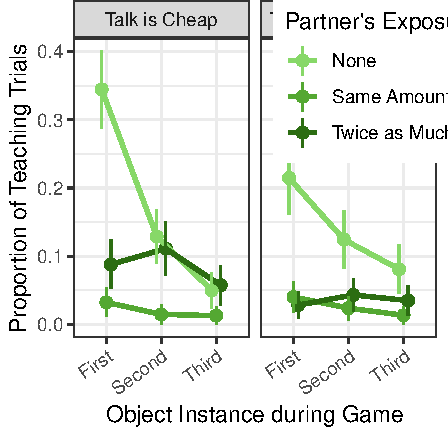
\includegraphics{figs/imp_teach-1} 

}

\caption[Rates of teaching across the partner exposure manipulation and appearances taken from speaker behavior during gameplay]{Rates of teaching across the partner exposure manipulation and appearances taken from speaker behavior during gameplay. Both the Talk is Cheap and Talk is Less Cheap condition yielded 30 points for correctly teaching a label, but the relative benefits of later labeling differed.}\label{fig:imp_teach}
\end{figure}
\end{CodeChunk}

\section{Model: Iterated Communication as Rational
Planning}\label{model-iterated-communication-as-rational-planning}

The results from this experiment are qualitatively consistent with a
model in which participants make their communicative choices to maximize
their expected utility from the reference game. We next formalize this
model to determine if these results are predicted quantitatively as
well.

\newcommand{\E}[1]{\mathbb{E}\left[ #1 \right]}

In a one-shot reference game maximizing expected utility is simply
choosing the action (\(a\)) that has the highest expected utility
\((\E{U})\). The expected utility depends both on the action itself, and
on the state of the two partners (\(s\)): For pointing, this expected
utility is independent of referent, defined entirely by our experimental
manipulation. In contrast, for speech, the utility varies with the
probability of partners sharing a common label for the referent.
Following other models in the Rational Speech Act framework, we use the
Luce Choice Axiom, in which each choice is taken in probability
proportional to its exponentiated utility (M. C. Frank \& Goodman,
2012). This choice rule has a single parameter \(\alpha\) that controls
the noise in this choice--as \(\alpha\) approaches 0, choice is random
and as \(\alpha\) approaches infinity choice is optimal:

\[ 
C\left(a;s\right) \propto e^{\alpha \E{U \left(s,a\right))}}
\]

To use this rule, agents have to estimate how likely they are to share a
common label (\(s\)). In our simulation, we assume for simplicity that
people have an accurate representation of their own knowledge. We thus
set each simulated participant's knowledge to the explicit recall
judgment made by a real participant in our experiments. To estimate
their partner's knowledge, participants can reason about their own
learning. Again for simplicity we model learning as a simple Bernoulli
process: Each exposure to novel label is like a flipping a coin with
weight \(p\), if it comes up heads, the label is learned. Having
observed their own learning outcomes, agents can infer their own
learning rate by determining the weight \(p'\) under which their
observed learning is most likely. Assuming that their partner would have
learned at the same rate, participants can then generate a probability
with which their partner would have learned each label by estimating the
probability that at least one of its \(n\) came up heads given learning
rate \(p'\): \(P\left(s^{+}\right)=1-p'\left( 1-p' \right)^{n}\).

In an iterated game, however, because actions taken on the current trial
can influence the state (\(s\)) on future trials, the optimal action to
take is not the one that optimizes the single trial's rewards, but
rather the one that optimizes the expected rewards that will accumulate
over all future trials (Kaelbling, Littman, \& Cassandra, 1998).

For the results reported here, we set \(\alpha = 2\) based on
hand-tuning, but other values produce similar results. \textbf{also the
discounting parameter}

We implemented a two-agent model of speaker and listener behavior in
this game based on partially observable Markov decision processes. The
speaker is given a target referent each trial and must signal to the
listener which object to select. Speakers send messages to the listener
by speaking, a low cost cue that relies on the listener's knowledge, or
by pointing, a higher cost cue that is unambiguous.

The speaker estimates the listener's knowledge. First, the speaker uses
Markov chain Monte Carlo to infer their own learning rate based on how
well they were able to learn a novel lexicon after N exposures. Then,
given the listener's degree of exposure, the speaker can use their own
learning rate to infer the probability that the listener would know any
given object-label mapping. Across trials, the speaker gains further
information about the listener through their selections, allowing them
to update their beliefs about the listener's knowledge state.

The model specifies the relative costs for each communicative modality.
On each trial, the speaker estimates the expected utility of each
modality by accounting for these costs, their own knowledge of the
object's label, and the probability that the listener knows the object's
label. The speaker then uses Luce's choice axiom to select a
communicative modality based on the expected utilities.

When estimating expected utility, the model sums the expected utility of
a given trial and any remaining trials for that particular object. This
allows the speaker to engage in planning by accounting for the way a
given message may induce knowledge changes and thus affect subsequent
expected utilities. Utilities were scaled using an exponential
discounter as a function of delay to give greater weight to immediate
rewards than subsequent rewards.

Crucially, speakers can also combine both communication cues, paying the
upfront cost of both, to produce a message that is both unambiguous and
informative. In this way, speakers are able to teach their partners
object-label mappings. A speaker that plans may thus infer that teaching
the listener, especially if there is an asymmetry in their knowledge
states, may have a high expected utility after accounting for remaining
trials where the speaker could use a less costly cue (i.e.~speech).
After producing both cues, the speaker also updates their own beliefs
about the partner's knowledge state to reflect this exposure.

\begin{CodeChunk}
\begin{figure}[H]

{\centering 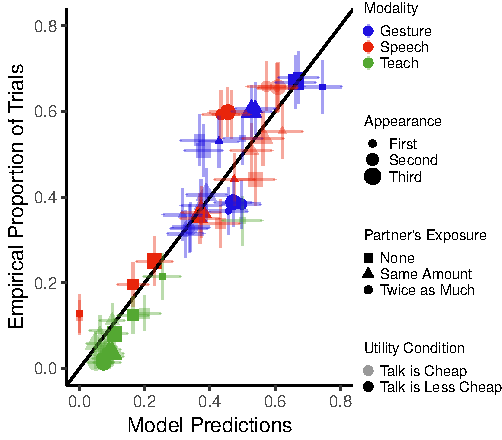
\includegraphics{figs/model_fit-1} 

}

\caption[Plot of the fit between model predictions and empirical data]{Plot of the fit between model predictions and empirical data.}\label{fig:model_fit}
\end{figure}
\end{CodeChunk}

\section{General Discussion}\label{general-discussion}

We showed that people tune their communicative choices to varying cost
and reward structures, and also critically to their partner's linguistic
knowledge--teaching when partners are unlikely to know language and many
more rounds remain. These data are consistent with the patterns shown in
our corpus analysis of parent referential communication and demonstrate
that such pedagogically-supportive input could arise from purely selfish
motives to maximize the utility of communicating successfully while
minimizing the cost of communication. We take these results as a proof
of concept that both the features of child-directed speech that support
learning as well as those that inhibit it may arise from a single
unifying goal: The desire to communicative efficiently.

Of course, this work is limited in a number of important ways. While our
task allows us to distill key pressures and manipulations, there are
signficant divergences from the corpus data-collecting environment as a
result. For one, there are fewer and less dynamic, reciporical
interactions between interlocutors and no time-constraints are imposed
on communication. Also, parents are likely aware of not just how much
language their children know, but \emph{what} their children know (at
least at a lexical level). Critical next steps in this line of work will
return back to the level of parent-child interaction.

Our framework is not specific to any particular language phenonmenon,
though we have focused on gesture-speech coocurrence here. Given the
right data or paradigm, our account should hold equally well when
explaining how other information-rich language input might arise in
naturalistic communication. Using coprus and experimental data, this
work validates the hypothesis that communicative pressure alone can lead
to supportive language input.

\section{References}\label{references}

\setlength{\parindent}{-0.1in} \setlength{\leftskip}{0.125in}

\noindent

\hypertarget{refs}{}
\hypertarget{ref-bloom2000}{}
Bloom, P. (2000). \emph{How children learn the meanings of words}. MIT
press: Cambridge, MA.

\hypertarget{ref-blythe2010}{}
Blythe, R. A., Smith, K., \& Smith, A. D. M. (2010). Learning times for
large lexicons through cross-situational learning. \emph{Cognitive
Science}, \emph{34}, 620--642.

\hypertarget{ref-brown1977}{}
Brown, R. (1977). Introduction. In C. E. Snow \& C. A. Ferguson (Eds.),
\emph{Talking to children: Language input and interaction}. Cambridge,
MA.: MIT Press.

\hypertarget{ref-eaves-jr2016}{}
Eaves Jr, B. S., Feldman, N. H., Griffiths, T. L., \& Shafto, P. (2016).
Infant-directed speech is consistent with teaching. \emph{Psychological
Review}, \emph{123}(6), 758.

\hypertarget{ref-frank2012}{}
Frank, M. C., \& Goodman, N. D. (2012). Predicting Pragmatic Reasoning
in Language Games. \emph{Science}, \emph{336}(6084), 998--998.

\hypertarget{ref-goldin-meadow2014}{}
Goldin-Meadow, S., Levine, S. C., Hedges, L. V., Huttenlocher, J.,
Raudenbush, S. W., \& Small, S. L. (2014). New evidence about language
and cognitive development based on a longitudinal study: Hypotheses for
intervention. \emph{American Psychologist}, \emph{69}(6), 588--599.

\hypertarget{ref-kaelbling1998}{}
Kaelbling, L. P., Littman, M. L., \& Cassandra, A. R. (1998). Planning
and acting in partially observable stochastic domains. \emph{Artificial
Intelligence}, \emph{101}, 99--134.

\hypertarget{ref-mcmurray2013}{}
McMurray, B., Kovack-Lesh, K. A., Goodwin, D., \& McEchron, W. (2013).
Infant directed speech and the development of speech perception:
Enhancing development or an unintended consequence? \emph{Cognition},
\emph{129}(2), 362--378.

\hypertarget{ref-newport1990}{}
Newport, E. L. (1990). Maturational Constraints on Language Learning.
\emph{Cognitive Science}, \emph{14}(1), 11--28.

\hypertarget{ref-newport1977}{}
Newport, E. L., Gleitman, H., \& Gleitman, L. R. (1977). Mother, I'd
rather do it myself: Some effects and non-effects of maternal speech
style. In C. A. Ferguson (Ed.), \emph{Talking to children language input
and interaction} (pp. 109--149). Cambridge University Press.

\hypertarget{ref-saffran2003}{}
Saffran, J. R., \& 2003. (2003). Statistical language learning:
Mechanisms and constraints. \emph{Current Directions in Psychological
Science}, \emph{12}(4), 110--114.

\hypertarget{ref-smith2008}{}
Smith, L. B., \& Yu, C. (2008). Infants rapidly learn word-referent
mappings via cross-situational statistics. \emph{Cognition}, \emph{106},
1558--1568.

\hypertarget{ref-smith2013}{}
Smith, L. B., \& Yu, C. (2013). Visual attention is not enough:
Individual differences in statistical word-referent learning in infants.
\emph{Language Learning and \ldots{}}, \emph{9}, 25--49.

\hypertarget{ref-vlach2013}{}
Vlach, H. A., \& Johnson, S. P. (2013). Memory constraints on infants
cross-situational statistical learning. \emph{Cognition}, \emph{127}(3),
375--382.

\hypertarget{ref-vogt2012}{}
Vogt, P. (2012). Exploring the robustness of cross-situational learning
under zipfian distributions. \emph{Cognitive Science}, \emph{36}(4),
726--739.

\hypertarget{ref-yurovsky2017}{}
Yurovsky, D. (2017). A communicative approach to early word learning.
\emph{New Ideas in Psychology}, 1--7.

\hypertarget{ref-yurovsky2016}{}
Yurovsky, D., Doyle, G., \& Frank, M. C. (2016). Linguistic input is
tuned to childrens developmental level. In \emph{Proceedings of the
annual meeting of the cognitive science society} (pp. 2093--2098).

\bibliographystyle{apacite}


\end{document}
